\documentclass[11pt]{article}
\usepackage[a4paper,top=2cm,bottom=2cm,left=2cm,right=2cm]{geometry}
\usepackage{graphicx}
\usepackage[italian,english]{babel}
\usepackage{amsthm, amsmath, amssymb}
\usepackage{setspace}\onehalfspacing
\usepackage[loose,nice]{units} %replace "nice" by "ugly" for units in upright fractions
\usepackage{frontespizio}
\usepackage[utf8x]{inputenc}
\usepackage[pdftex]{hyperref}
\usepackage{fancyhdr}
\usepackage{tabularx}
\usepackage{tikz}
\usepackage{amsmath}
\pagenumbering{gobble}
\tikzstyle{mybox} = [draw=black,thick, rectangle, rounded corners, inner ysep=7pt, inner xsep=7pt]
\selectlanguage{english}
\begin{document}
\begin{titlepage}
	
\begin{normalsize}
\begin{flushleft}
  \hspace{0pt} Moratello Matteo 1205720 \hspace{281pt} 06/13/2019\\

  \hspace{0pt} Master Degree in Computer Engineering\\
 
  \hspace{0pt} A.Y. 2018/19 Course of Computer Vision\\
[6mm]
\end{flushleft}
\end{normalsize}

	\begin{center}

\textsc{\huge \textbf{Project Report}} \\
[3mm]
\textsc{\large \textbf{AUTOMATIC LICENCE PLATE READING}} \\
[5mm]
\end{center} 
{ \setstretch{1.06}
Automatic licence plate reading require some intermediate processes in order to:
\begin{itemize}
\item Identify in the original image a window that contain the license plate (*);
\item Identify the licence plate in the window found;
\item Segment the licence plate and then extract all the digits;
\item Use a model of neural network in order to classify the digits found, at this point we have a string of the number of the licence plate.
\end{itemize}
(*) I used this approach in order to deal with all image of the dataset, in fact a focus on a window permit to extract licence plates well in images with very different size without change algorithm parameters.\\\\
\textbf{\large{1.1 - Identification of the license plate location using the sliding window approach}} \\
[1 mm]
The use of a sliding window is used in the program as a preprocessing of the image in order to detect subsequently the contours of the licence plate.
\\In order to detect the location of the licence plate in the best way, together with the sliding window a ORB extractor has been used. 
\\ The ORB extractor is used instead of SIFT because it is faster even if less precise, but since the images can also be very large, the time to calculate the descriptors can be very high and must be avoided especially for real-time systems.
\\ For first, the descriptors of a sample of a licence plate are extracted with ORB, then, once the window size is chosen, the latter is scrolled in y and x direction and the features are extracted with ORB.
\\ Using a matcher (BFMatcher in this case), all matches between descriptors of the window and the sample licence plate are computed. 
\\ In order to choose the best window that best cointain the licence plate, the average of distances of the matches is computed for each window. The best window will have the minimum mean of distances.
\\Considering the first image of the dataset (1.jpg), in the figure below are shown the matches between the sample plate and the first one window captured. It can be noticed that there are many false positives, in fact, the average of the distances of the correspondences is 93.6635 so it will certainly be discarded.
\begin{figure}[htbp]
\centering
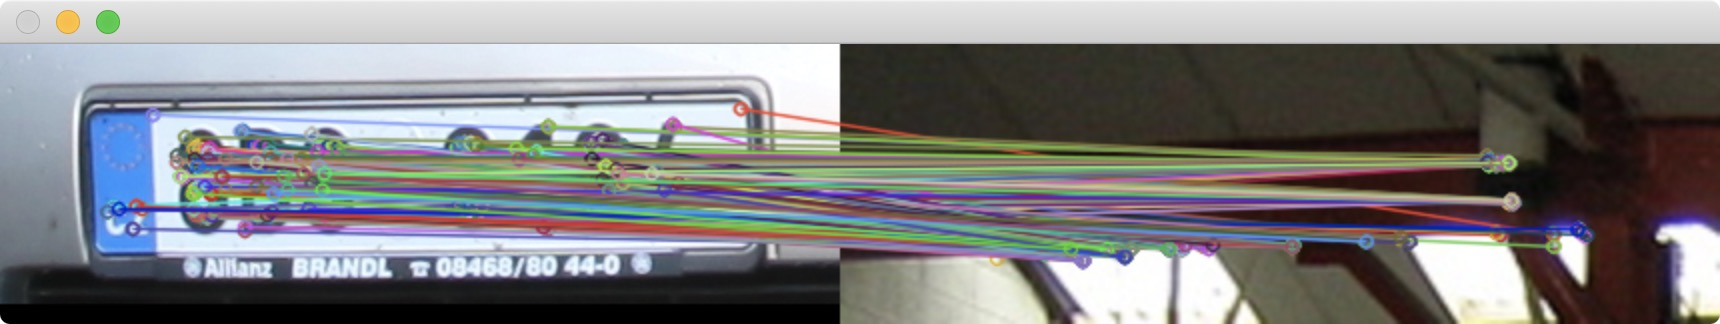
\includegraphics[totalheight=0.19\textwidth]{m1.jpg}
\caption{Matches between descriptors of the sample plate (on the left) and the first one window (on top-left of the image 1.jpg)}
\label{}
\end{figure}
\newpage
\noindent	
The next figure show instead the window that best contain the licence plate, in fact it's average of distances is 63.7841 , the minimum one between all the averages.
\begin{figure}[htbp]
\centering
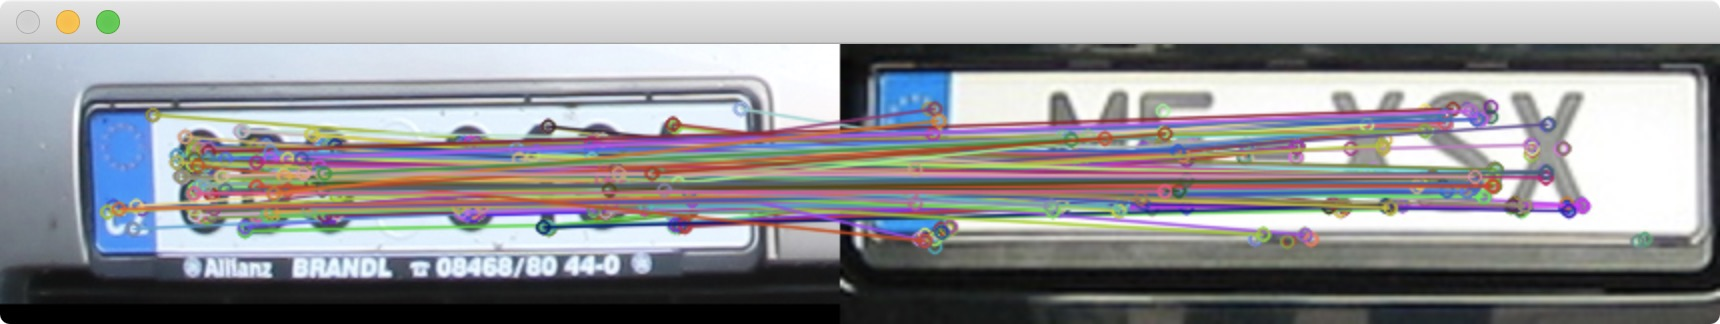
\includegraphics[totalheight=0.19\textwidth]{m2.jpg}
\caption{Matches between descriptors of the sample plate (on the left) and the best window found w.r.t. matches distances}
\label{}
\end{figure}
\\Below are shown two examples of windows that best contain the license plate for first two images of the dataset.
\begin{figure}[htbp]
\centering
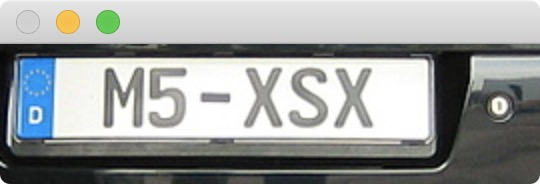
\includegraphics[totalheight=0.165\textwidth]{m3.jpg}
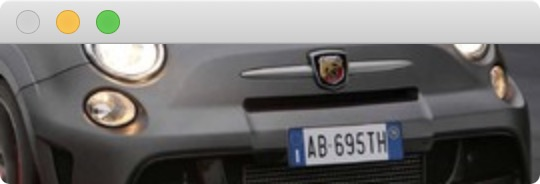
\includegraphics[totalheight=0.165\textwidth]{m4.jpg}
\caption{Best windows found for the first two images of the dataset. The best window is saved by adding some padding to the right to make sure you have taken the whole plate well.}
\label{}
\end{figure}
\\It can be noted that for two very different images in dimensions such as the first two, obviously the regions containing the targe will also be very different, this is the reason why the sliding window approach was used, in the image on the right (Fiat abarth) it was very complex to find the licence plate in the whole image because the dimensions were very small.
\\[3mm]
\textbf{\large{1.2 - Extract the license plate from the window that contain it}} \\
[1 mm]
In order to extract the licence plate from the window, a first process to apply on the window is Canny algorithm and then extract all edges from the image.
\\ Considering the window found in image 1.jpg, the following image shows the edges found with the Canny algorithm.
\begin{figure}[htbp]
\centering
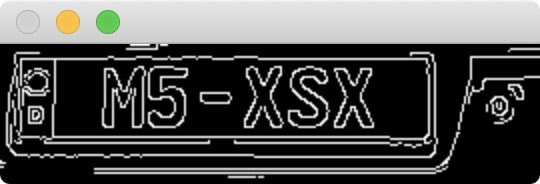
\includegraphics[totalheight=0.19\textwidth]{c.jpg}
\end{figure}
\\The next step is to find the contours of the edges found with the opencv findContours() function and then, for each contour found, a quadrilateral that contains it is constructed with the boundingRect() function.
\\At this point, the quadrilateral that best approximates the shape of a licence plate will be selected.
\\A first constraint is applied to the area of the quadrilateral which must be sufficiently large (I chose, rect.area() $>$ 1000) and two other constraints on the width/height ratio of the quadrilateral. This in fact must be within a certain range (I chose, 2.7 $<$= rect.width/rect.height $<$= 5.5).
\\After applying all the constraints to the various contours found, the Figure 4 shows the remaining quadrilaterals that are colored green.
\begin{figure}[htbp]
\centering
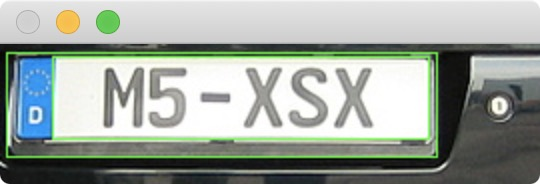
\includegraphics[totalheight=0.19\textwidth]{c1.jpg}
\caption{All rectangles found after applying constraints}
\label{}
\end{figure}
\newpage
\noindent	
Among all the rectangles found, the one with the smallest area is chosen and which will preferably contain only the characters of the plate. The final licence plate is shown in figure 5.
\begin{figure}[htbp]
\centering
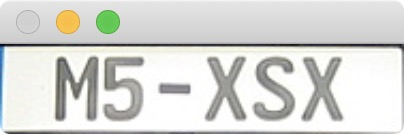
\includegraphics[totalheight=0.13\textwidth]{t.jpg}
\caption{Licence plate found}
\label{}
\end{figure}
\\ Considering briefly the image 2.jpg (in which the plate is a bit more challenging to find), the process just described with the images is shown below and it can be seen that the licence plate is extracted correctly.
\begin{figure}[htbp]
\centering
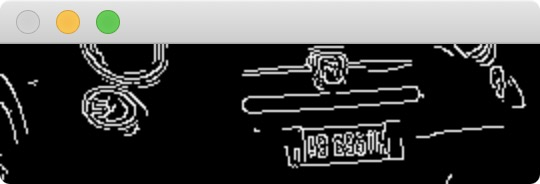
\includegraphics[totalheight=0.132\textwidth]{c3.jpg}
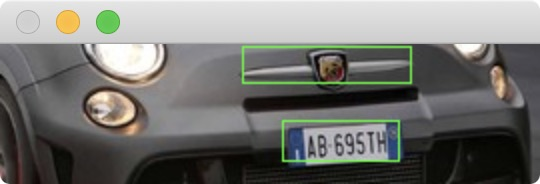
\includegraphics[totalheight=0.132\textwidth]{t1.jpg}
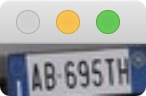
\includegraphics[totalheight=0.13\textwidth]{t2.jpg}
\end{figure}\\
\textbf{\large{1.3 - Extract digits from licence plate image}}\\
[1 mm]
In order to segment the licence plate, for first the image is converted in grayscale and then applied a threshold to the pixels intensities. The threshold transforms the image into a binary image, that is, with only the intensity values 0 or 255.
The figures below show the result of the process just described.
\begin{center}
\centering
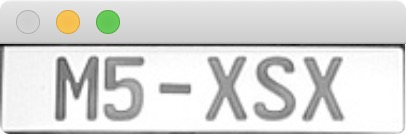
\includegraphics[totalheight=0.13\textwidth]{m.jpg}
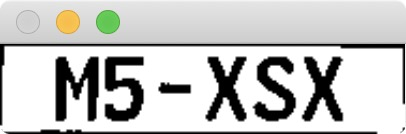
\includegraphics[totalheight=0.13\textwidth]{o.jpg}
\end{center}
The next step is to find the contours of the digits with the opencv findContours() function and for each contour found a quadrilateral is constructed that contains it, with the boundingRect() function.
\\ In order to discard shapes that aren't characters, some constraints are applied to quadrilaterals found.
\\A first constraint is applied to the area of the quadrilateral which must be sufficiently large (in this case, rect.area() $>$ 50) and two other constraints on the width/height ratio of the quadrilateral. This in fact must be within a certain range (in this case, 1.4 $<$= rect.width/rect.height $<$= 4.6).
\\ Another constraint applied in the selection of possible characters, is to discard the contours that contain more than 77\% of white pixels (intensity 255) on the total number of pixels.
\\The use of this constraint was necessary because in some digits/characters (like 8 or B), the ``holes" inside are identified as possible characters of the licence plate.
\\The figure 6 shows a possible case where this problem occurs.
\newpage
\begin{figure}[htbp]
\centering
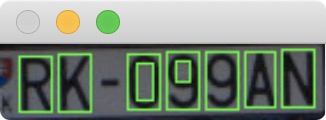
\includegraphics[totalheight=0.13\textwidth]{pro.jpg}
\caption{In this case the hole in digit 0 and in digit 9 are detected as chars}
\label{}
\end{figure}
\noindent
Figure 7 shows two results where all the characters are correctly segmented. The chars are then sorted according to their position in the x direction and saved in a vector of Mat.
\begin{figure}[htbp]
\centering
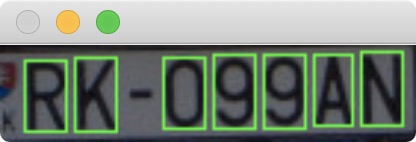
\includegraphics[totalheight=0.13\textwidth]{res.jpg}
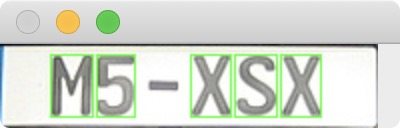
\includegraphics[totalheight=0.13\textwidth]{targa.jpg}
\caption{Characters of the licence plate are correctly segmented}
\label{}
\end{figure}
\\To get the correct input of the neural network, each character is resized to a size of 20x20 and the image has been made negative (1 - intensity of the pixel, for each pixel in the image).
\\For each plate, the images of the chars are concatenated in order to form a single image with the number of the licence plate and then saved in the folder ``licence\_plates".
\\Figure below shows the image of characters found in image 1.jpg.
\begin{figure}[htbp]
\centering

\includegraphics[totalheight=0.11\textwidth]{plate1.jpg}
\end{figure}
\\ The three processes seen so far are performed using methods of the PlateDetector class. Process 1.1 is contained in the \textbf{findPlateLocationInImage()} method, the process 1.2 in the \textbf{findBoundingOfPlate()} method and finally the process 1.3 in the \textbf{findCharsInPlate()} method. All the first part is write in c++ language.\\
\\\textbf{\large{2 - Use of a Neural Network to classify digits found}}\\
[1 mm]
In order to classify digits found it is been used a neural network using python Deep Learning library Keras. 
\\ The biggest problem in using neural networks is to find a fairly large and qualitative dataset. To classify license plate characters, the MNIST dataset cannot be used because it uses handwritten digits/characters.
\\ For the classification i used a dataset found on the net that includes characters and digits with different fonts (source: \href{https://archive.ics.uci.edu/ml/datasets/Character+Font+Images}{https://archive.ics.uci.edu/ml/datasets/Character+Font+Images}).
\\The dataset ARIAL.csv is a csv file that contains:
\begin{itemize}
\item Label: integer of the ascii code
\item Features: grayscale intensity of each pixels (400 features from 20x20 image)
\end{itemize}
Only the images relating to numbers or capital letters were extracted from the dataset, taking the number of classes to 36.
\\[1.5 mm]
\textbf{\large{2.1 - Architecture of the network}}
\\[1 mm]
The architecture of the network used is the one that best perform with MNIST dataset, in fact the images between the datasets are very similar.
\begin{itemize}
\item 2D convolution layer (number of filters: 18, size of each filter: 5x5)
\\ Spatial convolution over images
\item MaxPooling2D \\It is used for reduce the dimension and allow for assumptions to be made about features contained in the sub-regions binned. It reduces the computational cost by reducing the number of parameters to learn.
\item 2D convolution layer (number of filters: 26, size of each filter: 5x5)
\item MaxPooling2D 
\item 2D convolution layer (number of filters: 24, size of each filter: 5x5)
\item MaxPooling2D 
\item Flatten
\item Dense (Fully connected layer)
\item Dense (softmax)
\end{itemize}
Final layer returns the probability for each class that the input image belongs to that class.
\begin{figure}[htbp]
\centering
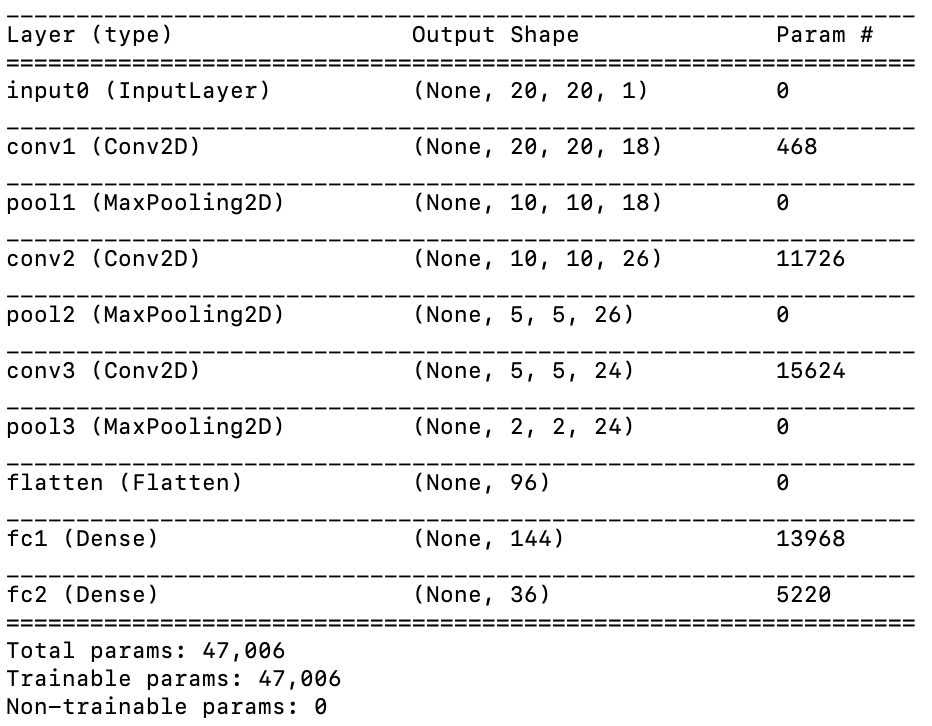
\includegraphics[totalheight=0.658\textwidth]{rete.jpg}
\caption{Summary of the Neural Network model}
\label{}
\end{figure}
\\\textbf{\large{2.1 - Training of the Neural Network}}
\\[1mm]
The image dataset composed of 8181 images was divided as follows:
\\ - 7362 training set (90\%)
\\ - 819 validation set (10\%)
\\ The neural network has been trained for 8 epochs, achieving an estimation error of 0.01 and training error of 0.0019.\\
Neural Network training is performed by the python program ``training\_model.py".
\\[1 mm]
\textbf{\large{2.2 - Classification}}
\\[1 mm]
In order to obtain a string of the number of the licence plate each single char extracted, from the concatenated image, is give in input to the neural network then all predicted characters are concatenated to form the final string. 
Example of correct classification is shown below (image 1.jpg).
\begin{center}
\centering

\includegraphics[totalheight=0.11\textwidth]{plate1.jpg}
\\Predict Labels: M5XSX
\\True Labels: M5XSX 
\end{center}
In the image 2.jpg the characters found was very small and not very detailed (with also some outliers), in fact there are many misclassified.
\begin{center}
\centering

\includegraphics[totalheight=0.11\textwidth]{plate2.jpg}
\\Predict Labels: AVY351 
\\True Labels: AB695T 
\end{center}
In general, the network obtained 91\% accuracy on the total of inputs (41 correct classify over 45).\\
Chars classification is performed by the python program ``classify\_chars.py"
\\[1 mm]
\textbf{\large{3 - Some results}}
\\[1 mm]
The c++ program load the txt file that contains the strings of the chars of all licence plates and show:
\\ - The original image with a green bounding box that highlights the licence plate found;
\\ - The number of the plate found in green. Some results are shown below.
\begin{figure}[htbp]
\centering
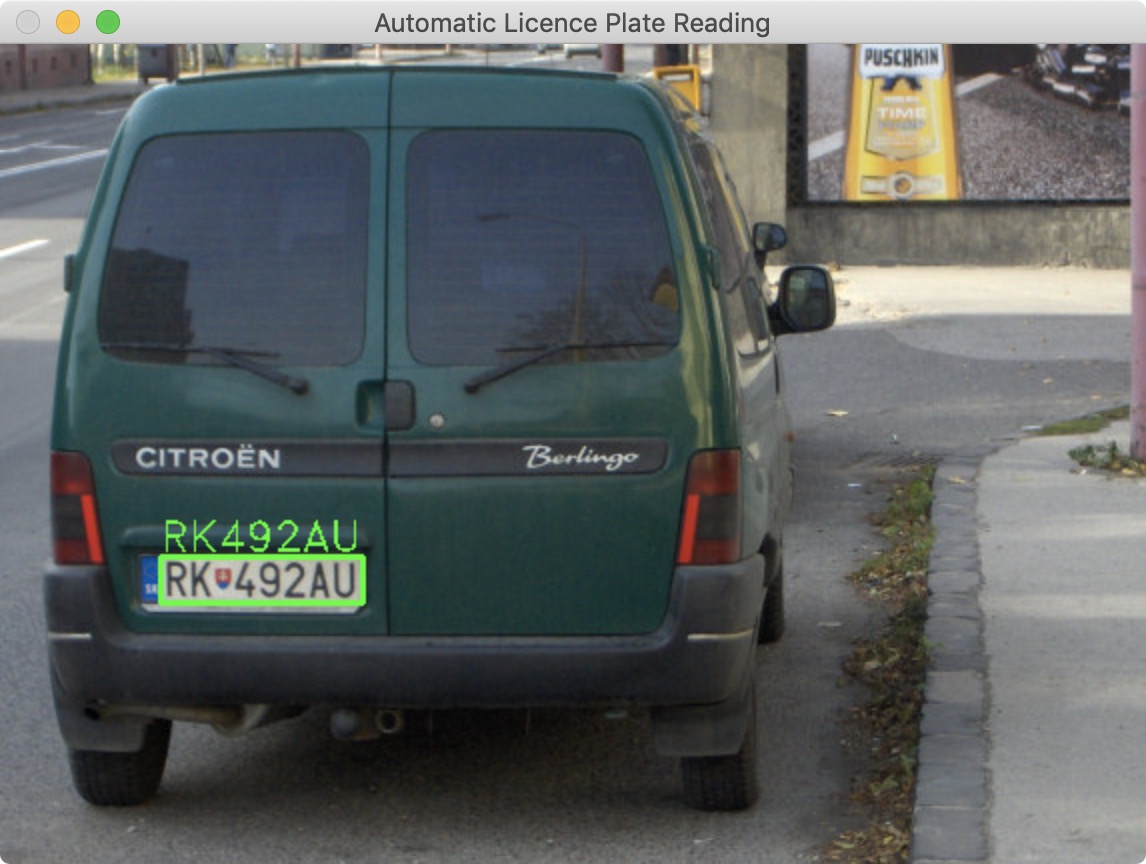
\includegraphics[totalheight=0.575\textwidth]{3.jpg}
\caption{Result of image 7.jpg (the number of the licence plate is also print in output)}
\label{}
\end{figure}
\begin{figure}[htbp]
\centering
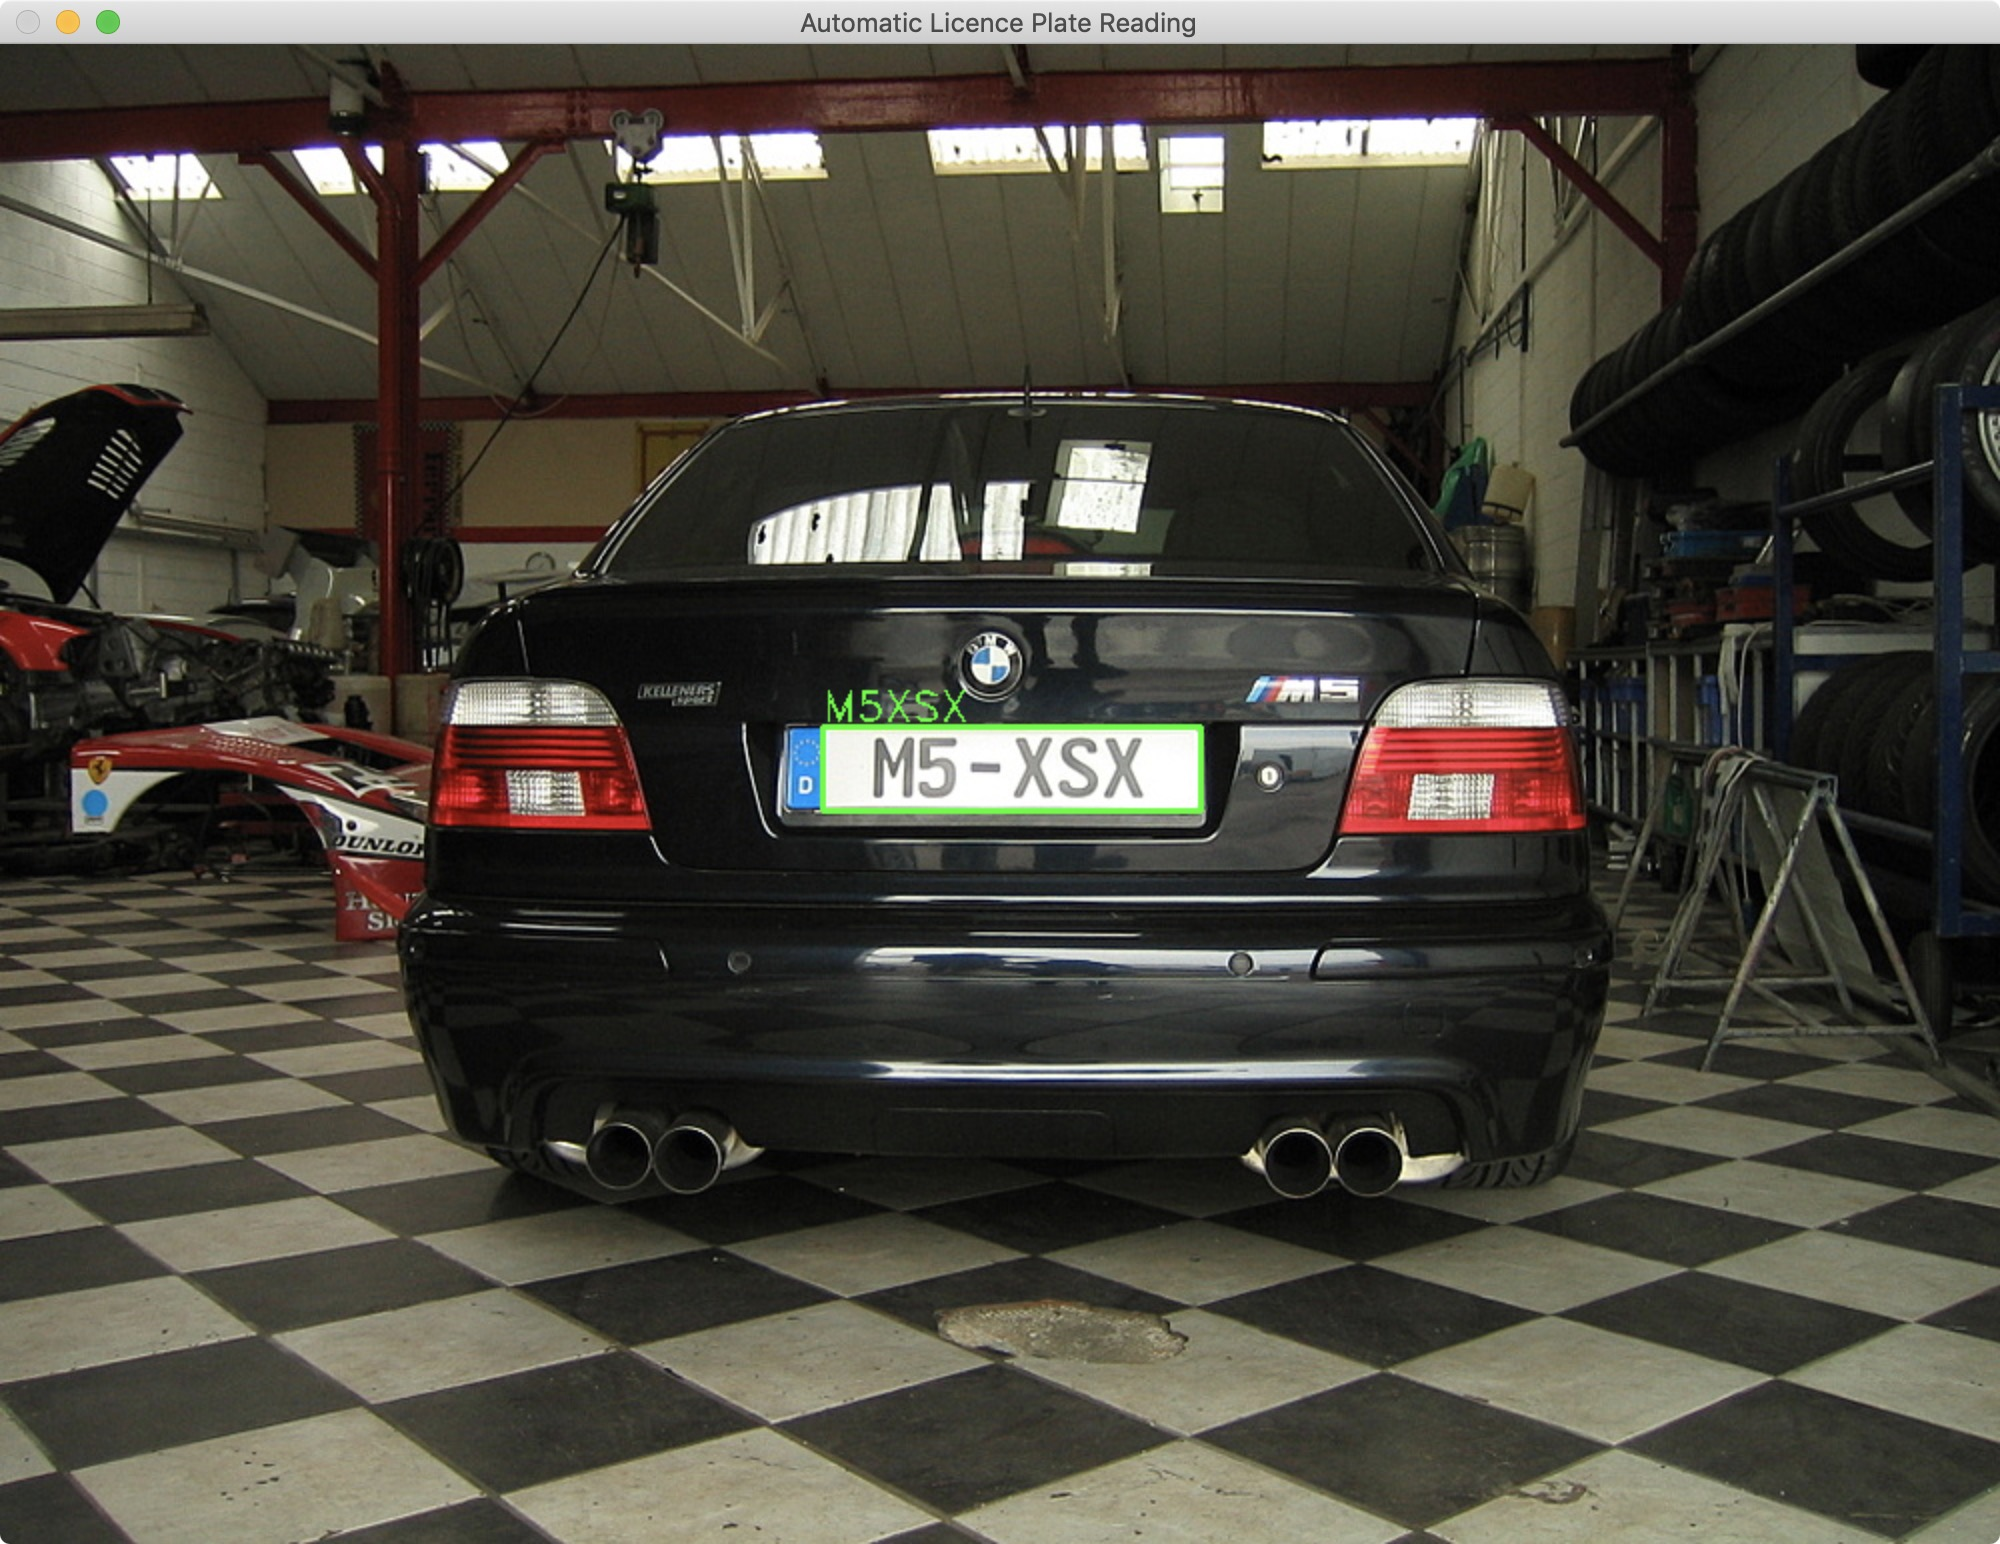
\includegraphics[totalheight=0.7\textwidth]{1.jpg}
\caption{Result of image 1.jpg}
\label{}
\end{figure}
\begin{figure}[htbp]
\centering
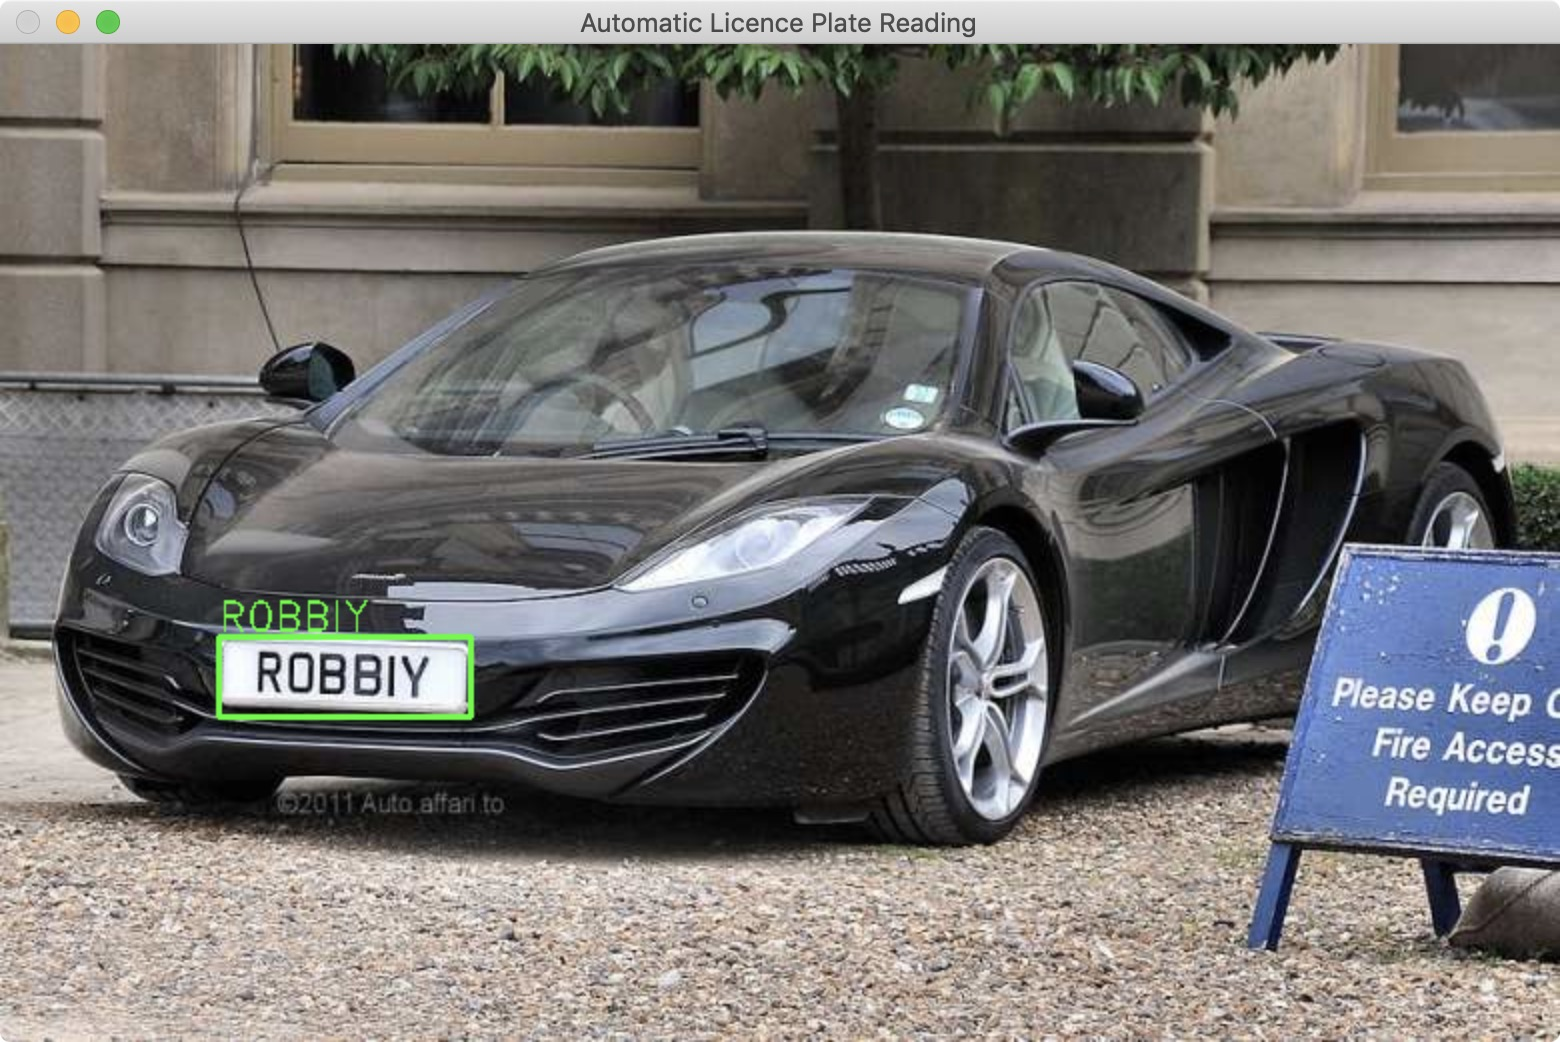
\includegraphics[totalheight=0.61\textwidth]{2.jpg}
\caption{Result of image 4.jpg}
\label{}
\end{figure}
\par}
\end{titlepage}
\end{document}